% Festlegung des Allgemeinen Dokumentenformats
\documentclass[a4paper,12pt,headsepline]{scrartcl}

% Umlaute unter UTF8 nutzen
\usepackage[utf8]{inputenc}

% Eigene packages
\usepackage{amsmath}
\usepackage{cite}

\usepackage{listings}
\usepackage{xcolor}
 
\definecolor{codegreen}{rgb}{0,0.6,0}
\definecolor{codegray}{rgb}{0.5,0.5,0.5}
\definecolor{codepurple}{rgb}{0.58,0,0.82}
\definecolor{backcolour}{rgb}{0.95,0.95,0.92}
 
\lstdefinestyle{mystyle}{
    backgroundcolor=\color{backcolour},   
    commentstyle=\color{codegreen},
    keywordstyle=\color{magenta},
    numberstyle=\tiny\color{codegray},
    stringstyle=\color{codepurple},
    basicstyle=\ttfamily\footnotesize,
    breakatwhitespace=false,         
    breaklines=true,                 
    captionpos=b,                    
    keepspaces=true,                 
    numbers=left,                    
    numbersep=5pt,                  
    showspaces=false,                
    showstringspaces=false,
    showtabs=false,                  
    tabsize=2
}
 
\lstset{style=mystyle}

% Variablen
%Variablen welche innerhalb der gesamten Arbeit zur Verfügung stehen sollen
\newcommand{\titleDocument}{Bachelor- / Masterarbeit}
\newcommand{\subjectDocument}{im Studiengang <Studiengang>}


% weitere Pakete
% Grafiken aus PNG Dateien einbinden
\usepackage{graphicx}

% Deutsche Sonderzeichen und Silbentrennung nutzen
\usepackage[ngerman]{babel}

% Eurozeichen einbinden
\usepackage[right]{eurosym}

% Zeichenencoding
\usepackage[T1]{fontenc}

\usepackage{lmodern}


% floatende Bilder ermöglichen
%\usepackage{floatflt}

% mehrseitige Tabellen ermöglichen
\usepackage{longtable}

% Unterstützung für Schriftarten
%\newcommand{\changefont}[3]{ 
%\fontfamily{#1} \fontseries{#2} \fontshape{#3} \selectfont}

% Packet für Seitenrandabständex und Einstellung für Seitenränder
\usepackage{geometry}
\geometry{left=3.5cm, right=2cm, top=2.5cm, bottom=2cm}

% Paket für Boxen im Text
\usepackage{fancybox}

% bricht lange URLs "schön" um
\usepackage[hyphens,obeyspaces,spaces]{url}

% Paket für Textfarben
\usepackage{color}

% Mathematische Symbole importieren
\usepackage{amssymb}

% auf jeder Seite eine Überschrift (alt, zentriert)
%\pagestyle{headings}

% erzeugt Inhaltsverzeichnis mit Querverweisen zu den Abschnitten (PDF Version)
\usepackage[bookmarksnumbered,pdftitle={\titleDocument},hyperfootnotes=false]{hyperref}
%\hypersetup{colorlinks, citecolor=red, linkcolor=blue, urlcolor=black}
%\hypersetup{colorlinks, citecolor=black, linkcolor= black, urlcolor=black}

% neue Kopfzeilen mit fancypaket
\usepackage{fancyhdr} %Paket laden
\pagestyle{fancy} %eigener Seitenstil
\fancyhf{} %alle Kopf- und Fußzeilenfelder bereinigen
\fancyhead[L]{\nouppercase{\leftmark}} %Kopfzeile links
\fancyhead[C]{} %zentrierte Kopfzeile
\fancyhead[R]{\thepage} %Kopfzeile rechts
\renewcommand{\headrulewidth}{0.4pt} %obere Trennlinie
%\fancyfoot[C]{\thepage} %Seitennummer
%\renewcommand{\footrulewidth}{0.4pt} %untere Trennlinie

% für Tabellen
\usepackage{array}
% Festlegung Art der Zitierung - Havardmethode: Abkuerzung Autor + Jahr
\bibliographystyle{alphadin}
% Paket für Zeilenabstand
\usepackage{setspace}
% für Bildbezeichner
\usepackage{capt-of}
% für Stichwortverzeichnis
\usepackage{makeidx}
\usepackage{cleveref}

\newtheorem{satz}{Satz}[section]
\newtheorem{definition}{Definition}[section]
\newtheorem{beweis}{Beweis}[satz]


% Indexerstellung
\makeindex
\setlength{\parindent}{0pt}





\begin{document}
% hier werden die Trennvorschläge inkludiert
%hier müssen alle Wörter rein, welche Latex von sich auch nicht korrekt trennt bzw. bei denen man die genaue Trennung vorgeben möchte
\hyphenation{
Film-pro-du-zen-ten
Lux-em-burg
Soft-ware-bau-steins
zeit-in-ten-siv
}


% Titelseite %
\thispagestyle{empty}


\begin{figure}[t]
 \centering
 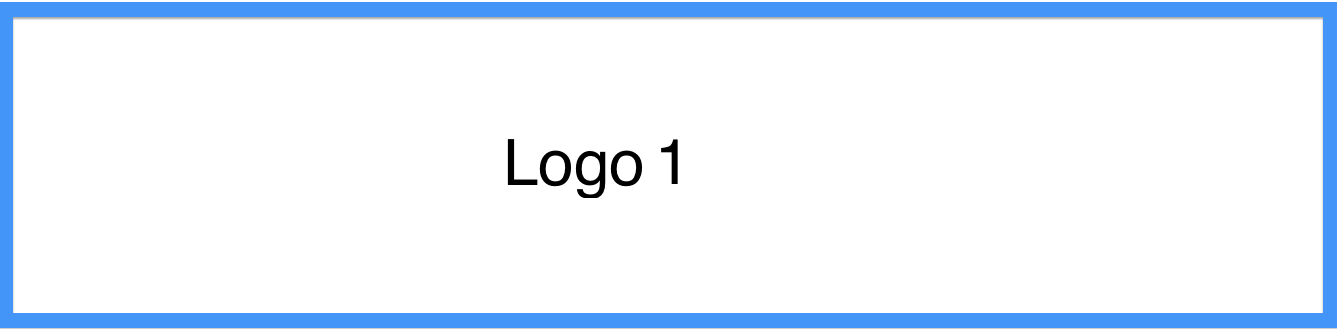
\includegraphics[width=0.6\textwidth]{abb/logo1}
~~~~~~~~~~
 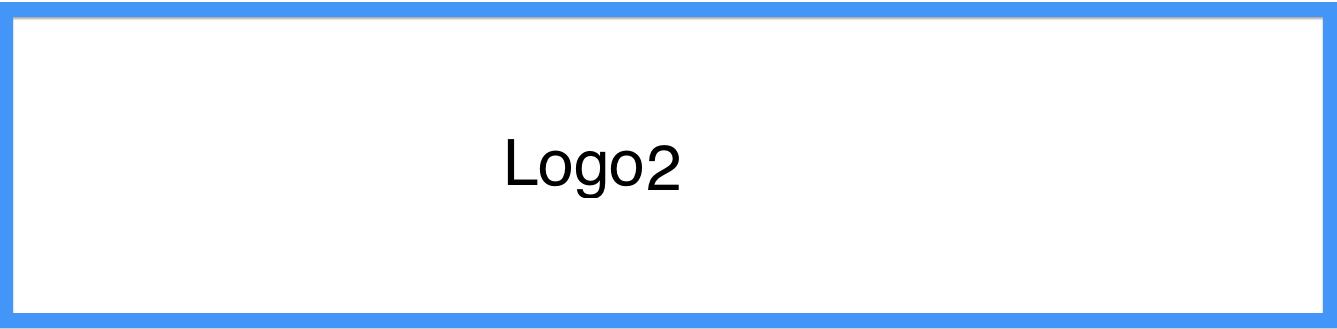
\includegraphics[width=0.3\textwidth]{abb/logo2}
\end{figure}


\begin{verbatim}


\end{verbatim}

\begin{center}
\Large{Fachhochschule <Name>}\\
\Large{- Campus <Name> -}\\
\end{center}


\begin{center}
\Large{Fakultät für <Fachrichtung>}
\end{center}
\begin{verbatim}




\end{verbatim}
\begin{center}
\doublespacing
\textbf{\LARGE{\titleDocument}}\\
\singlespacing
\begin{verbatim}

\end{verbatim}
\textbf{{~\subjectDocument~-~Schwerpunkt <Schwerpunktfach>}}
\end{center}
\begin{verbatim}

\end{verbatim}
\begin{center}

\end{center}
\begin{verbatim}

\end{verbatim}
\begin{center}
\textbf{zur Erlangung des akademischen Grades \\ Bachelor / Master of Science}
\end{center}
\begin{verbatim}






\end{verbatim}
\begin{flushleft}
\begin{tabular}{llll}
\textbf{Thema:} & & <Thema der Arbeit> & \\
& & \\
\textbf{Autor:} & & Name <name@mail.de>& \\
& & MatNr. 12345... & \\
& & \\
\textbf{Version vom:} & & \today &\\
& & \\
\textbf{1. Betreuerin:} & & Prof. Dr. X &\\
\textbf{2. Betreuer:} & & Prof. Dr. Y &\\
\end{tabular}
\end{flushleft}


% 1.5 facher Zeilenabstand
\onehalfspacing
\newpage

% Einleitung / Abstract
\section*{Zusammenfassung}

Diese Arbeit wird sich mit verschiedenen 
Optimierungsalgorithmen des Gradienten Abstiegsverfahren bei neuronalen Netzen beschäftigen
und diese auf Basis von Beispieldatensätzen evaluieren.
Hierbei wird eine Metrik definiert um die Ergebnis der einzelnen 
Optimierungsmethode zu vergleichen. 

Ein Optimierungsalgorithmus ist eine Möglichkeit
die Konvergenz der Fehlerfunktion $J(\theta)$ des neuronalen Netzes
beim Lernen zu verbessern. 

Hierbei wird auf den Lern Prozess des Neuronalen
Netzes eingegangen. Besonderen Fokus wird der ``Gradient Descent'',
zu Deutsch Gradienten Abstiegsverfahren, einnehmen, da dies die Grundlage
des Lernens darstellt. Dieser sucht im mehrdimensionalen Raum
die Minima der nichtlinearen Fehlerfunktion. Die Verbesserung 
dieser Suche machen sich die Optimierungsalgorithmen zur Aufgabe.  
Nach der theoretischen Aufarbeitung,
werden wir ein paar Eigenschaften über
diese Optimierungsmethoden annehmen
,um diese anhand der Testdaten zu überprüfen und mit der
Literatur zu vergleichen. 


\section*{Abstract}

This work will focus on explaning the different optimization methods of the gradient descent
algorithm of neural networks and evaluating them
on example datasets.
We will define a metric to be able to evaluate the performance 
of the different optimizer.

An optimization method is a way to improve the performance of the error 
function $J(\theta)$ of the neural network. 


Furthermore this work will give a detailed explanation of the learning process of Neural Networks
especially focusing on the Gradient Descent, which is the foundation of learning in neural networks.
This algorithm aims to find local minima in the Hyperplane of the non-linear error function. 
The optimization algorithms aim to improve this search. 
After the Theory, we will assume some properties about those optimization methods and test those assumptions
by evaluating the metrics of the neural networks. Then we will compare our results to
the literature


% Inhaltsverzeichnis anzeigen
\newpage
\tableofcontents


%%%%%%% EINLEITUNG %%%%%%%%%%%%
\newpage
\fancyhead[L]{\nouppercase{\leftmark}} %Kopfzeile links
\onehalfspacing

\section{Einleitung}\label{einleitung}

Hier steht die Einleitung der Arbeit... Lorem ipsum dolor sit amet, consetetur sadipscing elitr, sed diam nonumy eirmod tempor invidunt ut labore et dolore magna aliquyam erat, sed diam voluptua. At vero eos et accusam et justo duo dolores et ea rebum. Stet clita kasd gubergren, no sea takimata sanctus est Lorem ipsum dolor sit amet. Lorem ipsum dolor sit amet, consetetur sadipscing elitr, sed diam nonumy eirmod tempor invidunt ut labore et dolore magna aliquyam erat, sed diam voluptua. At vero eos et accusam et justo duo dolores et ea rebum. Stet clita kasd gubergren, no sea takimata sanctus est Lorem ipsum dolor sit amet.



\section{Theoretische Grundlagen}\label{Theoretische Grundlagen}


\subsection{Neuronale Netze}\label{Neuronale Netze}

Künstliche Neuronale Netze kurz KNNs sind der menschliche
Versuch das biologische Nervensystem nachzuahmen.
Sie basieren auf der Tatsache der Reizweitergabe. 
So wird ein Eingangsreiz von Rezeptoren aufgenommen 
und über verschiedene sogenannter Neuronen weitergegeben.
Durch diese Weitergabe wird das Signal verändert,
bis ein Ausgangssignal interpretiert werden kann. 
Diese Funktionsweise macht man sich bei künstlichen
Neuronalen Netzen zu nutze.
Der Eingangsreiz sind hier 
die sogenannten \grqq features\grqq{}, 
der Ausgangsreiz eine Klasse oder ein Wert
der interpretiert werden kann.
Wir wollen uns hier nun nur auf die \grqq Feed Forward\grqq{}
Netze fokussieren. Das bedeutet das Neuronen ihre Ausgabe
nur in eine Richtung schicken dürfen.


\begin{center}
 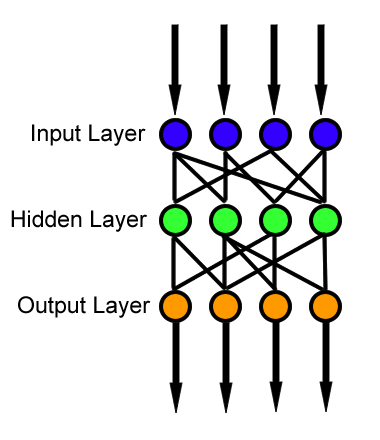
\includegraphics[width=0.4\textwidth]{abb/Feed_forward_neural_net.png}
 \captionof{figure}{Beispiel eines Feed Forward KNNs}
\end{center}


KNNs existieren in zwei Zuständen der Trainingsphase
und der Arbeitsphase. 
Die Trainingsphase ist die interessantere und wird in
dieser Arbeit beleuchtet. Hier werden durch Optimierung 
der Fehlerfunktion die Neuronen so "eingestellt" ,
dass sie einen möglichst gute Vorhersage treffen. 

Im Folgenden soll nun der Begriff des Neurons formalisiert 
werden, um die Verbesserungsmöglichkeiten des Gradienten
Verfahrens in Abschnitt \ref{Optimierungsmethoden} 
nachvollziehen zu können.

\begin{definition}
\cite[Kapitel 1.2]{BurkhardLenze.1997} Ein (\textbf{formales) Neuron} ist eine Funktion $\kappa: \mathbb{R}^n \rightarrow \mathbb{R}^m$ definiert durch:
\begin{itemize}
\item eine Aktivierungsfunktion $T:\mathbb{R} \rightarrow \mathbb{R}$
\item ein gewichteter Vektor $\vec{w} = \{w_1,w_2,...,w_n\}$
\item und eine Schwelle  $\Theta\in\mathbb{R}$.
\end{itemize}
Der Vektor $\vec{x} = (x_1,x_2,...,x_n)\in \mathbb{R}^n$ wird auf den Vektor $\vec{y} = (y,y,...,y)\in \mathbb{R}^m$ mit identischen Komponenten durch die folgende Rechenvorschrift abgebildet
\begin{align}
\kappa(\vec{x}):= (T(\sum\limits_{i=1}^n w_i x_i - \Theta),...,T(\sum\limits_{i=1}^n w_i x_i - \Theta))=\vec{y} \in \mathbb{R}^m
\end{align}   
\end{definition}
Hier seien ein paar Beispiele für Aktivierungsfunktionen angegeben
\begin{itemize}
\item Identität $T_I$
\begin{align*}
T(x):=x=T_I(x)
\end{align*}
\item Binary step
\begin{align*}
T(x) := \begin{cases} 0, \text{ for } x < 0 \\ 1, \text{ for } x \geq 0 \end{cases} =: T_1 (x)
\end{align*}
\item Sigmoid
\begin{align*}
T(x) := \frac{1}{1+e^{-x}} =: T_S(x)
\end{align*}
\item Tangens hyperbolicus
\begin{align*}
T(x) := \frac{1+tanh(x)}{2} =: T_H(x)
\end{align*}
\end{itemize}
Dies sind nur ein paar wenige Beispiele.
Jede Funktion $T:\mathbb{R}\rightarrow \mathbb{R}$
die $\lim\limits_{x \rightarrow -\infty}{T(x)}=0$ 
and $\lim\limits_{x \rightarrow \infty}{T(x)}=1$ erfüllt,
kann als Aktivierungsfunktion genutzt werden.

\begin{definition}
    \cite[Kapitel 2]{MichaelNielsen.Juni2019}
    Die \textbf{Fehlerfunktion} $J(\theta)$ eines Neuronalen Netzes ist eine 
    differenzierbare Funktion für die gilt:
    \begin{itemize}
        \item $J(\theta) = \frac{1}{n} \sum_x J_x$ wobei $x$ ein Eingabe Datum
        beschreibt.
        \item $J(\theta)$ lässt sich aus der Summe der Elemente des Ausgabe Vektors
        darstellen.
    \end{itemize}
\end{definition}

Die erste Eigenschaft bedeutet, dass die gesamte Fehlerfunktion 
sich auch durch die Fehlerfunkton der einzelnen Eingabe Daten darstellen lässt.
Diese Fehlerfunktion wird im nächsten Abschnitt minimiert werden, um
eine optimale Parameterbelegung der Gewichte $\vec{w}$ zu finden. 
Beispiele für eine solche Funktion wäre der 
mittlere quadratische Fehler.

\subsection{Gradient Descent}\label{Gradient Descent}

Der Gradient Descent oder zu Deutsch Gradienten Abstiegsverfahren
ist ein Weg eine Zielfunktion $J(\theta)$ parametrisiert durch $\theta \in \mathbb{R}^n$
zu minimieren. Man aktualisiert diese Parameter in Richtung des stärksten Abstiegs
der Zielfunktion $\nabla_\theta J(\theta)$. Die Lern Rate $\mu$ bestimmt
dabei die Größe der Aktualisierungsschritte. Das Verfahren folgt 
also der Richtung des Abstiegs der Oberfläche der Zielfunktion in ein Tal,
welches ein lokales Minimum
beschreibt. \cite[Kapitel 1]{Ruder.9152016} \\

Im Fall eines neuronalen Netzes ist die Zielfunktion $J(\theta)$ die
Fehlerfunktion des neuronalen Netzes. 
Wir brauchen einen solchen Algorithmus, da durch die Aktivierungsfunktion der Neuronen
wie in \ref{Neuronale Netze} beschrieben, die Fehlerfunktion nichtlinear wird und somit
die Minima sich nicht mehr analytisch berechnen lassen.
Um die Richtung des stärksten Abstiegs der Fehlerfunktion zu bestimmen, benötigen
wir den Gradienten.


\begin{definition}
    \cite{Konigsberger.2002}
    Der \textbf{Gradient} $\nabla$ der total differenzierbaren Funktion
    $f:\mathbb{R}^n \rightarrow \mathbb{R}$ im Punkt $a\in\mathbb{R}$ ist im
    Falle des Standard Skalar Produkts definiert durch:
    \begin{align}
        \nabla f := \frac{\partial f}{\partial x_{1}}\hat{e}_{1}+\cdots+\frac{\partial f}{\partial x_{n}}\hat{e}_{n}
    \end{align}
\end{definition}

In einfachen Worte gefasst, ist der Gradient die Ableitung einer mehrdimensionalen
Funktion, deren Funktionswerte man sich als Gebirge vorstellen kann.
Hierbei ist der Gradient in einen Punkt ein Vektor der in die Richtung des 
stärksten Anstiegs. \\
Um die Richtung des stärksten Abstiegs zu erhalten, welche wir beim Gradienten
Abstiegsverfahren benötigen, müssen wir nur den negativen Gradienten berechnen. \\\\
Mit diesem Wissen können wir nun den Standard gradient descent algorithmus definieren.

\begin{definition}
    \cite[Kapitel 2.1]{Ruder.9152016}
    Der sogenannte \textbf{batch gradient descent}, berechnet den Gradienten der 
    Kostenfunktion für den gesamten Datensatz. Jedes Update der Parameter ist definiert durch
    \begin{align}
        \theta = \theta - \eta \cdot \nabla_\theta J(\theta)
    \end{align}
    wobei $\eta$ die Lern Geschwindigkeit beschreibt.
\end{definition}


Als Algorithmus würde der batch gradient descent folgendermaßen aussehen.

\begin{lstlisting}[language=Python]
for i in range(nb_epochs ):
    params_grad = evaluate_gradient(loss_function , data , params)
    params = params  - learning_rate * params_grad
\end{lstlisting}

wobei \texttt{nb\_epochs} die Anzahl der Iterationen beschreibt. 
Diese Implementierung beschreibt die grundsätzliche Idee aber hat mehrere 
Nachteile. Da wir den Gradienten für den gesamten Datensatz berechnen ist 
diese Methode sehr langsam und nicht möglich für Datensätze, die nicht in den 
Arbeitsspeicher passen. Außerdem konvergiert dieser Algorithmus nur sehr langsam gegen
ein lokales Minimum. Zusätzlich ist die Wahl der perfekten Lern Geschwindigkeit oft
schwierig. \\

Zusätzlich benötigt man den Backpropagation Algorithmus um dieses Verfahren auf
ein gesamtes neuronales Netz anzuwenden. Dieser ist aber ebenfalls sehr komplex
und wird deshalb hier nicht behandelt. Er kann in \cite[Kapitel 2]{MichaelNielsen.Juni2019}
nachgelesen werden.

\subsection{Optimierungsmethoden}\label{Optimierungsmethoden}

Im vorherigen Abschnitt haben wir die Grundlagen des Gradienten Abstiegsverfahren
kennengelernt und gesehen, dass dieses Probleme mit sich bringt. Die folgenden
Optimierungsmethoden verbessern das grundsätzliche batch gradient descent Verfahren
in die ein oder andere Richtung.


\subsubsection{Stochastic Gradient Descent}\label{Stochastic Gradient Descent}

\begin{definition}
    \cite[Kapitel 2.2]{Ruder.9152016}
    Der Aktualisierungsschritt des \textbf{stochastic gradient descent} ist definiert durch 
    \begin{align}
        \theta = \theta - \eta \cdot \nabla_\theta J(\theta;x^{(i)};y^{(i)})
    \end{align}
\end{definition}

Der Unterschied zum \textbf{batch gradient descent} ist nur, dass der Aktualisierungsschritt
für jedes einzelne Datum ausgeführt wird. Das macht den 
Algorithmus wesentlich schneller, aber lässt ihn ebenfalls 
stärker schwanken, während er ein lokales Minimum sucht. Dies kann
positiv wie negativ sein, da eine solche Schwankung 
den Algorithmus Ebenen schneller überwinden lässt, aber manchmal
auch Minima überspringen lässt. Um eine gut Konvergenz zu gewährleisten,
erweitert man den Algorithmus noch um zwei Eigenschaften.

\begin{itemize}
    \item Die $x^{(i)}, y^{(y)}$ werden jede Iteration zufällig angeordnet
    \item Die Lern Geschwindigkeit $\eta$ wird linear verkleinert. 
\end{itemize}

Der stochastic gradient descent kann durch folgende Eigenschaft noch 
erweitert werden.

\begin{align}
    \theta = \theta - \eta \cdot \nabla_\theta J(\theta;x^{(i:i+n)};y^{(i:i+n)})
\end{align}

Nun wird nicht mehr für jedes einzelne Datum der Gradient berechnet, sondern
für einen Teilmenge der Größe $n$. In mancher Literatur, wird 
dieser Algorithmus noch einmal extra als \textbf{Mini-batch gradient descent} benannt.
\cite[Kapitel 2.3]{Ruder.9152016}. In den Implementierungen wird hier jedoch meist 
keine Unterscheidung mehr getroffen. \cite{FrancoisChollet.}

\subsubsection{Adagrad}\label{Adagrad}

Der Adagrad Algorithmus erweitert den Stochastic Gradient Descent noch weiter.
Bisher wurde die Lern Geschwindigkeit $\eta$ entweder konstant gelassen oder linear verkleinert.
Die Lern Geschwindigkeit hat somit keinen Bezug auf die Trainingsdaten. Hier setzt Adagrad an.
Er verändert die Lern Geschwindigkeit im Verhältnis zur Dichte des jeweiligen Parameters.

Deshalb hängt der Algorithmus diesmal auch von jedem einzelnen Elemente von $\theta$,
 bezeichnet als $\theta_i$ ab.
 
\begin{definition}
    \cite[Kapitel 4.3]{Ruder.9152016}
    Der \textbf{Adagrad} Algorithmus ist definiert durch den Aktualisierungsschritt
    \begin{align}
        \theta_{t+1,i} = \theta_{t,i} - \frac{\eta}{\sqrt{G_{t,ii}+\epsilon}} \cdot g_{t,i}
    \end{align}
    wobei $g_{t,i}$ definiert ist durch
    \begin{align}
        g_{t,i} = \nabla_{\theta_t} J(\theta_{t,i})
    \end{align}
    und $G_t \in R^{d\times d}$ ist eine diagonal Matrix, wobei die Diagonalelemente $i,i$, die 
    Summe der Quadrate der Gradienten zum zugehörigen Parameter $\theta_i$ bis zum Zeitpunkt
    t sind und $\epsilon > 0$ 
    
\end{definition}

Dies bringt eine große Erleichterung im Vergleich zu den bisherigen Algorithmen.
Durch die automatische und variable Anpassung der Lern Geschwindigkeit gewinnt man 
eine einfachere Implementierung und bessere Ergebnisse. 
\\\\
Adagrad hat jedoch einen Nachteil, durch die quadrierten summierten Gradienten
unter dem Bruch konvergiert die Veränderung der Parameter gegen null.
Deshalb kann Adagrad situationsbedingt auch schlechter als 
die bisherig vorgestellten Algorithmen sein. 

\subsubsection{Adam}\label{Adam}
\cite{DiederikP.KingmaandJimmyLeiBa.2015}
Adaptive Moment Estimation (Adam) ist ein Weiterer Alg


\section{Evaluation}\label{Evaluation}

In diesem Kapitel wollen wir uns jetzt mit der Analyse der einzelnen 
Optimierungsmethoden beschäftigen. Mithilfe des vorherigen Kapitel wollen
wir nachweisen, dass ein theoretisch besserer Algorithmus auch wirklich besser 
arbeitet. Was in diesem Fall ``besser'' bedeutet soll ebenfalls geklärt werden.

\subsection{Test Datensatz} \label{Test Datensatz}

Um ein neuronales Netz zu bewerten, brauchen wir zunächst einige Test Daten,
hierbei werden die beiden frei verfügbaren Datensätze, der \textit{Boston House Price}
Datensatz und der \textit{Breast Cancer} Datensatz, benutzt. Beide sind im \textit{scikit-learn}
Paket \cite{scikit-learn} enthalten. 

\subsubsection{Boston House Price} \label{Boston House Price}

Der \textit{Boston House Price} Datensatz besteht aus einem Regressionsproblem.
Das bedeutet, dass wir eine reelle Zahl mit unserem Netz voraussagen wollen, nämlich den
Preis eines Hauses in Boston. Damit das das  Netz lernen kann gibt es einige 
explanatorische Variablen wie unter anderem

\begin{itemize}
    \item \textbf{CRIM}: Die Verbrechensrate pro Kopf.
    \item \textbf{RM}: Die Anzahl der Räume im Haus.
    \item \textbf{TAX}: Steuer die auf das Grundstück gezahlt werden muss.
    \item \textbf{DIS}: gewichteter Abstand zum Zentrum von Boston. 
\end{itemize}

Mit diesen, insgesamt 13 Hilfsvariablen soll das Netz den Haus Preis voraussagen.

\begin{figure}[htbp] 
    \centering
       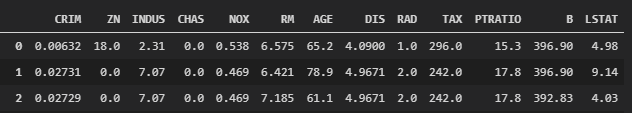
\includegraphics[width=1.0\textwidth]{abb/BostonBeispiel.PNG}
    \caption{Beispiel des Boston Datensatzes}
    \label{fig:BostonBeispiel}
\end{figure}


\subsubsection{Breast Cancer} \label{Breast Cancer}

Der \textit{Breast Cancer} Datensatz hingegen besteht aus einem binären Klassifikationsproblem.
Das bedeutet, dass das Netz nur ``ja'' oder ``nein'' kodiert als eins oder null, voraussagen
soll. Hierbei bedeutet ein Ja, dass diese Person Brustkrebs hat. Hier gibt es 
wieder einige explanatorische Variablen, die dem Netz helfen sollen zu lernen.
Diese sind Eigenschaften des Nukleus einer entommenen Brustzelle


\begin{itemize}
    \item \textbf{radius}: Radius des Nukleus
    \item \textbf{texture}: Standardabweichung der Graustufenwerte
    \item \textbf{symmetry}: Symmetrie des Nukleus
    \item \textbf{smoothness}: Lokale Abweichung der Radius Länge
\end{itemize}

Insgesamt besteht der Datensatz aus 30 solchen Variablen.

\begin{figure}[htbp] 
    \centering
       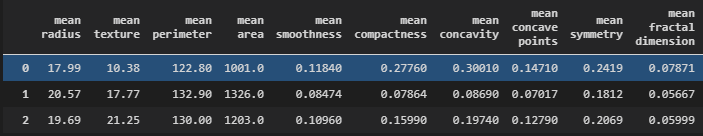
\includegraphics[width=1.0\textwidth]{abb/BreastCancerBeispiel.PNG}
    \caption{Beispiel des Breast Caner Datensatzes}
    \label{fig:BreastCancerBeispiel}
\end{figure}

\subsection{Metrik} \label{Metrik}

Bevor wir mit dem Vergleich der verschiedenen Optimierungsmethoden der Gradienten
beginnen können, brauchen wir ein Maß für die Güte eines Ergebnisses. 
Dafür müssen wir eine Metrik definieren. Sinnvoll ist es ein neuronales Netz
daran zu messen, wieviel es richtig bewertet hat. Richtig ist im Falle des \textit{Breast Cancer}
Datensatzes einfach ob das Netz ja zu ja und nein zu nein gesagt hat. Im Falle 
des \textit{Boston House Price} Datensatzes ist richtig, wenn der Abstand vom
vorhergesagten zum echten Preis möglichst klein ist. Dies gibt uns eine 
Vielzahl von Metriken die diese Voraussetzungen erfüllen.\\

Günstiger Weise benötigen wir bereits durch das Training des neuronalen Netzes 
eine Gütefunktion die angibt ob sich die Parameter in die richtige Richtung bewegen.
Diese ist die in Abschnitt \ref{Neuronale Netze} bereits besprochene Fehlerfunktion des 
Netzes. Diese sollte unsere erste Form einer Metrik sein um das Neuronale Netz zu bewerten.

Für den \textit{Boston House Price} Datensatz ist diese Fehlerfunktion die
\textit{mittlere quadratische Abweichung}.

\begin{definition}
    \cite[S.344]{Fahrmeir.2016} Die \textbf{mittlere quadratische Abweichung} für eine Stichprobe $x_1,...,x_n$
    mit Schätzwerten $\hat{x}_1,...,\hat{x}_n$ ist definiert durch
    \begin{align}
        \frac{1}{n}\sum\limits_{i=1}^{n} (\hat{x}_i-x_i)^2
    \end{align}
\end{definition}

Dies ist die typische Fehlerfunktion für Regressionsprobleme. Man mag sich fragen
warum diese quadriert wird und nicht der absolute Abstand zum echten Wert genommen
wird, wie vorher überlegt. Diese Funktion ist aber diejenige aus der wir den Gradienten
berechnen wollen, also muss sie differenzierbar sein, was das Quadrat gewährleistet.\\

Für den \textit{Breast Cancer} Datensatz ist diese Funktion jedoch unzureichend, da 
nur null oder eins im Wertebereich der mittleren quadratischen Abweichung vorkommen würden.
Da es sich hier um ein binäres Klassifikationsproblem handelt, eignet sich die \textit{binäre Kreuzentropie}.

\begin{definition}
    \cite{Rubinstein.2004} Die \textbf{binäre Kreuzentropie} für eine Stichprobe $x_1,...,x_n$
    mit Schätzwerten $\hat{x}_1,...,\hat{x}_n$ ist definiert durch
    \begin{align}
        \frac{1}{n}\sum\limits_{i=1}^{n} x_i log(\hat{x}_i) + (1-x_i)log(1-\hat{x}_i)
    \end{align}
    wobei $log$ der natürliche Logarithmus ist.
\end{definition}

Diese Fehlerfunktion ist geeignet für Wertebereiche zwischen null und eins. Also genau 
passend für ein zwei Klassen Klassifikationsproblem. \\

Diese beiden Fehlerfunktionen geben uns eine erste Idee für die Güte des neuronalen 
Netzes und deren Prädiktion und damit auch einen Indikator, welches
Netz den besseren Optimierungsalgorithmus besitzt, wenn sonst alle Parameter 
gleich bleiben. 
Zusätzlich nehmen wir um mehr Vergleichbarkeit zu schaffen eine weitere Fehlerfunktion hinzu,
die nur der Evaluierung der besseren Optimierungsmethode dient und nicht 
für das Gradienten Abstiegsverfahren genutzt wird.
Im Falle des \textit{Boston House Price} Datensatzes benutzen wir noch den 
\textit{Mittleren absoluten Fehler}.

\begin{definition}
    Der \textbf{Mittlere absolute Fehler} für eine Stichprobe $x_1,...,x_n$
    mit Schätzwerten $\hat{x}_1,...,\hat{x}_n$ ist definiert durch
    \begin{align}
        \frac{1}{n}\sum\limits_{i=1}^{n} | \hat{x}_i-x_i |
    \end{align}
\end{definition}

Dies ist die intuitivere Definition des Fehlers und ist somit geeignet um die
Optimierungsmethoden zu vergleichen.

Für den \textit{Breast Cancer} Datensatz benutzen wir zusätzlich die \textit{Accuracy},
um die Ergebnisse des neuronalen Netzes vergleichbarer zu machen.

\begin{definition}
    Die \textbf{Accuracy} einer Stichprobe der Größe $n$ ist definiert durch 
    \begin{align}
        Accuracy = \frac{\text{Anzahl korrekter Voraussagen}}{n}
    \end{align}
\end{definition}

Diese ist ebenfalls das intuitivere Verständnis der Güte eines neuronalen Netzes und hilft
somit bei der Auswertung der Optimierungsalgorithmen.

\subsection{Programm} \label{Programm}
 
Für einen Aufbau eines solchen Netzes und die Anwendung des Gradienten Abstiegsverfahrens
gibt es bereits verschiedenste Frameworks. Diese stehen vor Allem in \textit{Python} zur
Verfügung, da diese eine der vorrangigen KI Sprachen ist. Aus diesem Grund 
wird das folgende Programm für die Auswertung der Optimierungsalgorithmen, auf unseren
zwei Test Datensätzen, ebenfalls in \textit{Python} implementiert sein. 

\subsubsection{Frameworks}

Um uns die Arbeit zu erleichtern und um die Optimierungsalgorithmen, sowie das 
neuronale Netz nicht selbst implementieren zu müssen benutzen wir einige Frameworks.

\begin{itemize}
    \item \textbf{Keras} \cite{chollet2015keras}: Ein Framework, um neuronale Netze durch ein ``Baustein'' artiges 
        Prinzip aufzubauen. 
    \item \textbf{Scikit-learn} \cite{scikit-learn}: Ein Framework, welches viele machine learning-
        sowie Vorverarbeitungsalgorithmen als Funktionsaufruf zur Verfügung stellt.
    \item \textbf{Pandas} \cite{mckinney-proc-scipy-2010}: Ein Framework, was uns 
        tabellenartige Datenstrukturen zur Verfügung stellt, welche die Weiterverarbeitung vereinfachen.
    \item \textbf{Numpy} \cite{numpy}: Ein Framework für wissenschaftliche Berechnungen 
        in Python, wie zum Beispiel Matrizenmultiplikation.  
\end{itemize}

\subsubsection{Aufbau} \label{Aufbau}

Die Idee hinter dem Aufbau des Python Programms war eine Objekt orientierte Klassenlandschaft
zu erstellen, um möglichst allgemein die verschiedenen Optimierungsalgorithmen an unterschiedlichen 
Neuronalen Netzen und Datensätzen zu testen. Das folgende UML-Diagramm veranschaulicht
diese Prämisse.

\begin{figure}[htbp] 
    \centering
       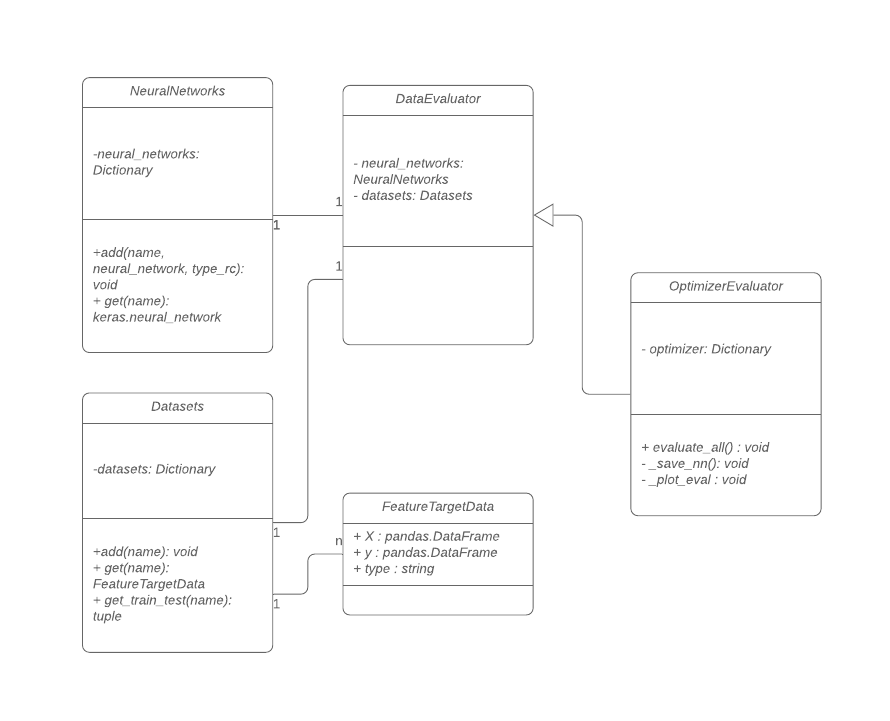
\includegraphics[width=1.0\textwidth]{abb/STI_fertig.png}
    \caption{UML-Diagramm des Python Programms}
    \label{fig:UML}
\end{figure}

Die wichtigste Klasse hier ist der \texttt{DataEvaluator}. Er verallgemeinert 
das Konzept einer Testklasse, die Neuronale Netze zu bestimmten Datensätzen auswertet.
Was dabei ausgewertet wird, wird allgemein gehalten. Die konkrete Implementierung erfolgt 
in der \texttt{OptimizerEvaluator} Klasse, die mit der \texttt{evaluate\_all} Methode
die eigentliche Auswertung der Optimierungsalgorithmen übernimmt. Diese 
erbt von \texttt{DataEvaluator} und besitzt somit dessen Attribute, die vom Typ
\texttt{NeuralNetworks} und \texttt{Datasets} sind.

Diese besitzen jeweils ein dictionary
Attribut, in dem sie nach dem key value Prinzip ihre jeweiligen Inhalte speichern.
In \texttt{Datasets} werden die Auszuwertenden Datensätze gespeichert. Diese Datensätze
sind vom Typ \texttt{FeatureTargetData}. 

Dieser neue Datentyp wird benötigt
um später einfach zwischen explanatorischen Variablen und Zielvariablen zu unterscheiden.
In \texttt{X} werden die explanatorischen Variablen gespeichert und in \texttt{y} die Zielvariable.
Zusätzlich speichern wir die Art der Vorhersage, die auf dem Datensatz möglich ist.
Also entweder ``Regression'' oder ``Klassifikation''. Wir benötigen diese Information, 
um später die richtigen Metriken auszuwählen. Wie in Abschnitt \ref{Metrik} erläutert, 
benutzen wir verschiedene Metriken für Regressions- und Klassifikationsprobleme.

In der \texttt{Neural Networks} Klasse werden die neuronalen Netze, die 
uns das Keras Framework zur Verfügung stellt gespeichert. Dabei wird nur deren
Struktur gespeichert. Die Gewichte werden erst später angepasst, wenn wir das Netz
auf einen Datensatz trainieren. 

\subsubsection{Netzstruktur}

Oftmals steht und fällt ein neuronales Netz mit seiner vorher festgelegten
Struktur. Diese kann das Netz nicht selbst lernen, sondern muss vom Menschen 
vorgegeben werden. Da unser Hauptfokus jedoch der Vergleich der Optimierungsalgorithmen
ist, und nicht der Aufbau eines perfekten neuronalen Netzes,
ist die Netzstruktur eher zweitrangig. Zusätzlich sind die 
Testdatensätze eher einfachere Probleme, die auch simple 
neuronale Netzstrukturen gut lernen können. Wichtig ist nur, dass wir immer 
den gleichen Netzaufbau für jede Optimierung benutzen um Vergleichbarkeit zu schaffen. 

Im folgenden soll die Netzstruktur, die wir für die Regressionsprobleme
des \textit{Boston House Price} Datensatzes benutzen erläutert werden.

\begin{lstlisting}[language=Python]
_regression_NN_boston = Sequential()
_regression_NN_boston.add(
    Dense(units=160, activation='relu', input_shape=(13,)))
_regression_NN_boston.add(Dense(units=64, activation='relu'))
_regression_NN_boston.add(Dense(units=1, activation='linear'))
\end{lstlisting}

Diese Definition ist für das \textit{Keras} Framework gedacht.
Hier definiert man jede Ebene des Netzes nacheinander. 
Wir initialisieren das Netz mit dem \texttt{Sequential} Konstruktor.
Das bedeutet, dass wir ein normales feed forward Netz bauen wollen,
wie in Abschnitt \ref{Neuronale Netze} erläutert. 
Nun fügen wir die erste Ebene des Netzes hinzu. Diese ist \texttt{Dense}, 
was bedeutet, dass jedes Neuron mit jedem verknüpft ist.
Außerdem sind insgesamt 160 Neuronen in dieser Ebene. 
Die Anzahl der Neuronen ist üblicherweise ein Indikator dafür, wie komplex das 
Netz ist und vor Allem wie komplex das Problem ist, welches das Netz versucht
zu lösen. Für diese einfache Problematik sollten 160 Neuronen jedoch ausreichen
\\

In dieser Ebene verwenden wir die nichtlineare Aktivierungsfunktion \textit{Relu},
wie in Definition \ref{Def:formales Neuron} bereits erläutert, wird diese nichtlineare
Funktion benötigt um nichtlineare Probleme zu lösen und macht somit das 
Gradienten Abstiegsverfahren erst notwendig.
Da es sich hier um eine innere Schicht eines feed forward Netzes handelt ist die
Wahl von Relu eindeutig. Diese hat sich in den letzen Jahren als beste 
Aktivierungsfunktion für innere Schichten herausgestellt. \cite[S. 226]{Goodfellow.2016}
Der Parameter \texttt{input\_shape} gibt an wie viele explanatorische Variablen
dem Netz zugeführt werden. Wie in Abschnitt \ref{Boston House Price} besprochen,
besitzt der \textit{Boston House Price} Datensatz 13 explanatorische Variablen.
Mit diesem Prinzip wird noch eine innere Schicht hinzugefügt und schließlich 
die Ausgabeschicht die nur aus einem einzigen Neuron besteht, da wir hier die
Zahl für den Preis erwarten.\\

Für den \textit{Breast Cancer} Datensatz ergibt sich ein ähnlicher Aufbau.

\begin{lstlisting}[language=Python]
_classification_NN_breast_cancer = Sequential()
_classification_NN_breast_cancer.add(
    Dense(40, input_shape=(30,), activation='relu'))
_classification_NN_breast_cancer.add(Dense(20, activation='relu'))
_classification_NN_breast_cancer.add(Dense(1, activation='sigmoid'))
\end{lstlisting}

Nur das hier in der Ausgabeschicht die \textit{Sigmoid} Funktion verwendet wird, 
da wir eine Zahl zwischen null und eins erwarten. Nämlich die Wahrscheinlichkeit
für Brustkrebs. 

\subsection{Auswertung} \label{Auswertung}

Nun ist alles bereit um die verschiedenen Netze mit unterschiedlichen Optimierungsalgorithmen
zu trainieren und diese anschließend mit den Metriken aus Abschnitt \ref{Metrik}
zu bewerten. 

\subsubsection{Erwartungen} \label{Erwartungen}

Wir werden die drei vorgestellten Algorithmen 
\begin{itemize}
    \item Stochastic Gradient Descent
    \item Adagrad
    \item ADAM
\end{itemize}

anwenden und ihre Performance mithilfe der Metriken messen. Der \textit{Stoachstic Gradient Descent}
ist dabei der simpelste Algorithmus. Also würden wir erwarten, dass dieser die schlechtesten 
Ergebnisse liefert. \textit{Adagrad} und \textit{ADAM} sind ähnlich, jedoch 
benutzt ADAM noch mehr Informationen als Adagrad. \textit{ADAM} sollte somit 
die beste Performance haben. Adagrad sollte aber auch nicht schlecht sein, da 
beide Datensätze eher klein sind und somit eine adaptive Anpassung der Gewichte
wichtig ist.

\subsubsection{Boston House Price Auswertung} \label{Boston House Price Auswertung}

Für die Auswertung des \textit{Boston House Price} Datensatzes haben wir den \textit{MSE} (in der Abbildung \ref{fig:BHPAuswertung} unter Loss) und den \textit{MAE} 
als Metrik ausgewählt. Umso niedriger diese Werte sind, desto besser hat das Netz den Hauspreis 
vorausgesagt. 

\begin{figure}[htbp] 
    \centering
       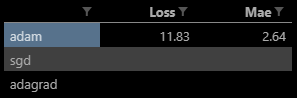
\includegraphics[width=0.6\textwidth]{abb/boston_score.png}
    \caption{Boston House Price Auswertung}
    \label{fig:BHPAuswertung}
\end{figure}

In Abbildung \ref{fig:BHPAuswertung} ist klar zu erkennen das keine Werte unter 
den beiden Optimierungsmethoden \textit{SGD} und \textit{Adagrad} eingetragen wurden.
Das liegt daran dass diese Optimierungsalgorithmen nicht konvergiert sind. 

\begin{figure}[htbp] 
    \centering
       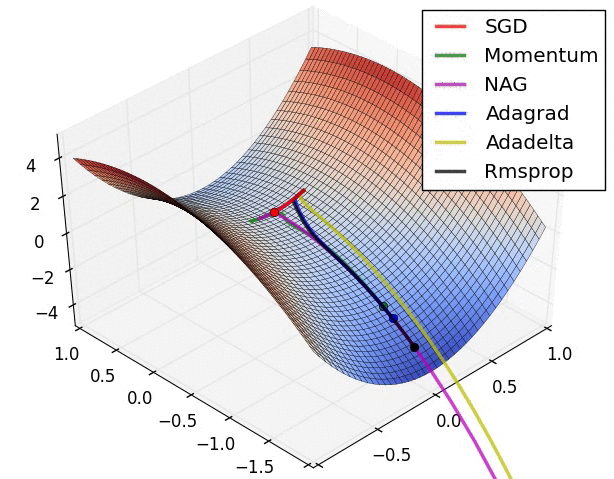
\includegraphics[width=0.6\textwidth]{abb/VisualizationDivergenz.PNG}
    \caption{Visualisierung Divergenz - Quelle: \url{https://imgur.com/a/Hqolp}}
    \label{fig:Divergenz}
\end{figure}

In Abbildung \ref{fig:Divergenz} sehen wir die Oberfläche für ein solches Ergebnis.
Die Algorithmen starten offensichtlich in der Nähe eines Sattelpunkts und folgen einem
unendlichen Abstieg. Bei \textit{ADAM} passiert dies jedoch nicht. Dieser ist offensichtlich
wesentlich robuster gegenüber solchen Sattelpunkten. 
Ein anderer Grund für eine solche Divergenz könnte beim Stochastic Gradient Descent auch eine 
unpassende Lernrate $\eta$ sein. Oft können solche Divergenzen auch durch eine schlechte 
Parametrisierung des Lernraums entstehen. Dadurch, dass die Distanzen in einem 13 dimensionalen 
Raum sehr groß werden, können solche Divergenzen begünstigt werden. 
Die Variablen wurden jedoch vor dem Training normalisiert, weswegen dieser Grund ausgeschlossen
werden kann. 

\subsubsection{Breast Cancer Auswertung} \label{Breast Cancer Auswertung}

Für die Auswertung des \textit{Breast Cancer} Datensatzes benutzen wir die Metriken 
der \textit{binären Kreuzentropie} (in Abbildungen \ref{fig:BCAuswertung} als Loss benannt)
und die Accuracy. Die binäre Kreuzentropie soll dabei möglichst klein sein, wogegen die Accuracy
möglichst nah bei eins sein sollte, um ein besseres Ergebnis zu liefern.  

\begin{figure}[htbp] 
    \centering
       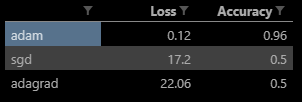
\includegraphics[width=0.6\textwidth]{abb/breast_cancer_score.PNG}
    \caption{Breast Cancer Auswertung}
    \label{fig:BCAuswertung}
\end{figure}

Hier sehen wir ebenfalls, dass \textit{ADAM} die besten Ergebnisse zeigt. 
Die beiden anderen Optimierungsalgorithmen zeigen deutlich stärkere Fluktuationen auf.
Interessant ist hier, dass der \textit{Stochastic Gradient Descent} besser performt als \textit{Adagrad}.
Dies liegt wahrscheinlich an der wie in Abschnitt \ref{Adagrad} besprochenen Summierung der Gradienten,
welche \textit{Adagrad} irgendwann stoppen lässt ein Minimum zu suchen.


\subsubsection{Vergleich mit der Literatur} \label{Vergleich mit Literatur}

In der Literatur ist ebenfalls oft die Rede von \textit{ADAM} als go-to Optimierungsalgorithmus,
da er sehr robust ist und man kein Parametertuning benötigt um gut Ergebnisse zu bekommen. 
\textit{Adagrad} hat offensichtlich Probleme mit Konvergenz, wie wir ebenfalls nachweisen konnte und ist 
daher nur in seltenen Fällen benutzbar, da die adaptive Anpassung der Parameter ebenfalls 
von \textit{ADAM} besser durchgeführt wird. Jedoch scheint der \textit{Stochastic Gradient Descent}
ebenfalls sehr wirkungsvoll zu sein. Das Problem ist jedoch, dass der \textit{Stochastic Gradient Descent}
eine gute Lernrate braucht, die nicht offensichtlich ist, wie wir in der Auswertung gesehen haben.
Außerdem braucht man eine gute Initialisierung und der Algorithmus braucht deutlich länger.
\cite[Abschnitt 4.10]{Ruder.9152016}

\section{Fazit}\label{Fazit}

Zusammengefasst kommt die Literatur auf ein ähnliches Ergebnis, wie die Auswertung 
der zwei Datensätze. Der \textit{ADAM} Optimierungsalgorithmus ist ein robuster und 
einfach zu benutzender Algorithmus, der für die meisten neuronalen Netze gute Ergebnisse liefert. 
Das macht ihn am besten für eine Erstauswertung, wie wir sie hier auch hatten. 
Wenn die Struktur der Daten nicht bekannt ist und man schnelle Ergebnisse braucht 
sollte man den \textit{ADAM} Algorithmus wählen. Jedoch kann es in besonderen 
Fällen von Vorteil sein einen anderen Algorithmus wählen, wie den \textit{Stoachastic
Gradient Descent}. Jedoch ist das sehr datenabhängig.

% einfacher Zeilenabstand
\singlespacing
% Literaturliste soll im Inhaltsverzeichnis auftauchen
\newpage
\addcontentsline{toc}{section}{Literaturverzeichnis}
% Literaturverzeichnis anzeigen
\renewcommand\refname{Literaturverzeichnis}
\bibliography{Hauptdatei}

% Eidesstattliche Erklärung
\newpage
\addcontentsline{toc}{section}{Eidesstattliche Erklärung}
\section*{Eidesstattliche Erklärung}
\thispagestyle{empty}

\begin{verbatim}

\end{verbatim}

\begin{LARGE}Eidesstattliche Erklärung zur Seminararbeit\end{LARGE}
\begin{verbatim}


\end{verbatim}
Ich versichere, die von mir vorgelegte Arbeit selbstständig verfasst zu haben. Alle Stellen, die wörtlich oder sinngemäß aus veröffentlichten oder nicht veröffentlichten Arbeiten anderer entnommen sind, habe ich als entnommen kenntlich gemacht. Sämtliche Quellen und Hilfsmittel, die ich für die Arbeit benutzt habe, sind angegeben. Die Arbeit hat mit gleichem Inhalt bzw. in wesentlichen Teilen noch keiner anderen Prüfungsbehörde vorgelegen.



\begin{displaymath}
% use packages: array
\begin{array}{ll}
Unterschrift:~~~~~~~~~~~~~~~~~~~~~~~~~~~~~~~~~~~~~~~~~~
& Ort, Datum:~~~~~~~~~~~~~~~~~~~~~~~~~~~~~~~~~~~~~~~~~~
\end{array}
\end{displaymath}


\end{document}
